\documentclass[a4paper,twocolumn]{jsarticle}
%\documentclass[a4j,twocolumn]{jarticle} % 'jsarticle' が使えない場合はこちらを利用

% 上記 documentclass のオプションは自由に追加してもよい。

%%%%%%%%%%%%%%%%%%%%%%%%%%%%%%%%%%%%%%%%%%%%%%%%%%%%%%%%%%%%%%%%%%%%%%%%%%%%%%
%%% ページ設定 (この項目は論文著者は編集しないこと。)

% 芸術科学会学術会議用スタイルパッケージ
\usepackage{artsci-conf-j} 

%%%%%%%%%%%%%%%%%%%%%%%%%%%%%%%%%%%%%%%%%%%%%%%%%%%%%%%%%%%%%%%%%%%%%%%%%%%%%%
%%% パッケージ一覧 (必要なパッケージを任意に追加してよい)

\usepackage{amsmath, amssymb}	% AMS-LaTeX
\usepackage[dvipdfmx]{graphicx}	% 「graphics」パッケージに変更してもよい。
\usepackage{float}		% 図表が記述位置から飛ばないためのパッケージ
\usepackage{url}

%%%%%%%%%%%%%%%%%%%%%%%%%%%%%%%%%%%%%%%%%%%%%%%%%%%%%%%%%%%%%%%%%%%%%%%%%%%%%%
%%% マクロ一覧 (必要なマクロをこの部分に記述)

\newcommand{\bA}{\mathbf{A}}
\newcommand{\bB}{\mathbf{B}}



%%%%%%%%%%%%%%%%%%%%%%%%%%%%%%%%%%%%%%%%%%%%%%%%%%%%%%%%%%%%%%%%%%%%%%%%%%%%%%
%%% 図ファイルのパス設定

\graphicspath{{fig/}}

%% タイトル,概要,キーワードなど
%%%%%%%%%%%%%%%%%%%%%%%%%%%%%%%%%%%%%%%%%%%%%%%%%%%%%%%%%%%%%%%%%%%%%%%%%%%%%%
%%% タイトル、著者、所属、概要

% 日本語タイトル
\jtitle{
レトロネーザルアロマを利用した \\
味覚の拡張(\LaTeX 版)
}

% 英語タイトル
\etitle{
Expressive Japan \\
Sample Style (\LaTeX Version)
}

% 日本語著者
% 共著者氏名の間隔は ~ や \quad 等で適宜調節のこと。
\jauthor{
濱家陸\({}^\dagger\) \quad
}

% 英語著者
\eauthor{
Riku Hamaie\({}^\dagger\) \quad
}

% 日本語所属
\jaffiliation{
\(\dagger\) 東京工科大学 ~~~
	〒192-0982 東京都八王子市片倉町1404-1 \\
\(\ddagger\) 東京工科大学メディア学部 ~~~
	〒192-0982 東京都八王子市片倉町1404-1
}

% 英語所属
\eaffiliation{
\(\dagger\) Graduate School of Bionics, Computer and Media Sciences,
	Tokyo University of Technology \\
\(\ddagger\) School of Media Science,
	Tokyo University of Technology
}

% 連絡先電子メールアドレス
% (
% このサンプルでは「@」を2バイト文字にすることで対応してある。)
\email{
m01172238c@edu.teu.ac.jp
}

% 日本語概要
\jabstract{
嗅覚は味の知覚に密接に関わり影響を与えている.
風味に着目し,密接に関わっている口内から入る香り(レトロネーザル)を利用した.
レトロネーザルで感じた風味は味を感じ方に大きな影響を与えると考え,舌で感じる味覚ではなく嗅覚から感じる風味に焦点をあてた実験を検証した。
口の中からの嗅覚刺激を用いて香りを提示することで, 風味を与えることができるのではないかと考え,香りを閉じこめた直径 3 センチメートルのゼリーを食べることで,風味を想起させることが出来るかを検討した.
被験者に風味を感じることができるかを判断してもらい,風味提示ゼリーの有用性を示した.	
}

% 英語概要
\eabstract{
This article is to provide LaTeX sample for posting of ``Expressive Japan''.
This sample is created with emphasis on consistency with the sample of
the journal of the Society of Art and Science.
}

% 日本語キーワード
\jkeyword{
嗅覚, 味覚, 香り, 風味
}

% 英語キーワード
\ekeyword{
LaTeX, article, template, society
}


%%%%%%%%%%%%%%%%%%%%%%%%%%%%%%%%%%%%%%%%%%%%%%%%%%%%%%%%%%%%%%%%%%%%%%%%%%%%%%
% ここより論文本体
\pagestyle{empty}

\begin{document}
\maketitle

\section{はじめに}
\subsection{人間の嗅覚}
\label{subsec:intro}
人間の食べる時に使う感覚は舌による味覚だけではなく,嗅覚,視覚,聴覚,触覚の五感すべて
によって刺激から感じる. 本研究では,その中でも味覚に注目して,味覚に関係性が深い嗅覚に
着目した.嗅覚は,食べ物の香りを感じる時にとても敏感に働く感覚である.食べる前に香りを
嗅ぐと,食欲を増大させる.他に,食事の良し悪しや好き嫌いを判断する時にも,必要となる感
覚である.そのため,物を食べるときは,味覚で感じている前に食に対しての情報を感じとる感
覚である.その情報が味覚の感覚に影響を与え,感じ方を変化させるため「味」に大きな影響を
与えていると言われている.嗅覚には 2 つの嗅覚経路を通ることで嗅状皮細胞にたどり着く.一
つ目は鼻から入る経路で,一般的に匂いを嗅ぐときに使う嗅感覚である.二つ目は口から入り鼻
から抜けて出ていく経路で,食べ物を食べた時や口の中に入れた時に生じるものである.嗅覚は
嗅状皮細胞が特定の化学物質に触れ合うことで香りを認識する.この二つの嗅覚から味や匂いの
感覚を認識している.


\subsection{オルソネーザルアロマとレトロネーザルアロマ}
嗅覚には図\ref{kyukaku}で示したようにオルソネーザルと言われる鼻から入る香りとレトロネーザルと
言われる口から入り鼻から抜ける香りの2つがある.鼻をつまむと味がしなくなる現象や風邪な
ど鼻の不具合により味がしなくなる現象から嗅覚は味覚に影響があることが分かる.オルソネー
ザルの場合は,鼻から生じる単独の感覚であり,香りに特化した知覚である.一方,レトロネー
ザルは口内から入るため,味覚や感覚,触覚も加わることから複数の感覚が連動して新たな風味
が形成される.


\begin{figure}[t]
    \centering
    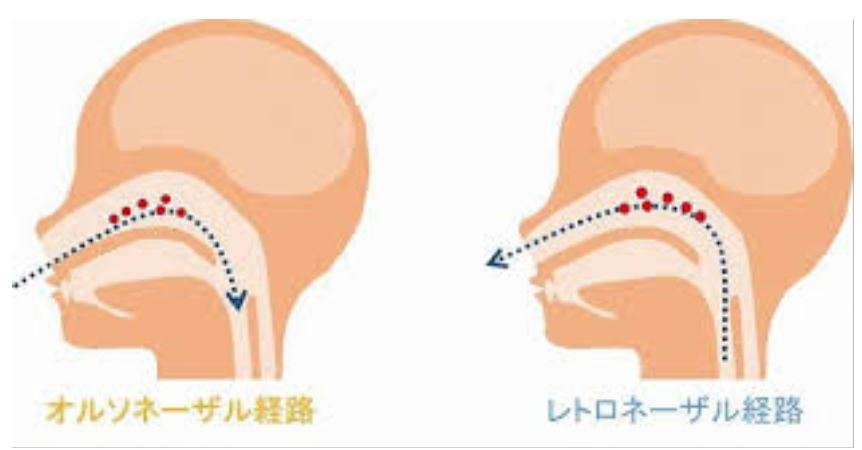
\includegraphics[width = 0.7\columnwidth]{kyukaku.JPG}
    \caption{オルソネーザルとレトロネーザル}
    \label{kyukaku}
  \end{figure}


\subsection{研究の目的}
レトロネーザルはオルソネーザルよりも複数の感覚から風味を感じやすいと考える.そのため
レトロネーザルを利用し,口の中から香りを与え嗅覚に刺激を与えることで風味を感じさせるこ
とが出来ると考えた.このように嗅覚刺激による風味,味覚への変化を検証する研究は存在する
が,食べられるものを使い香りを与えるものは少ない.チューブによって香りを嗅覚に与えるデ
バイスが多いため,食べれるものでの仕組みを作り出すことで口の中にチューブを入れるなどの
問題点を解決できるのではないかと考えた.


本稿では,口の中に香りを与える方法として,アガーで作成したゼリーの中に香りを閉
じこめたものを用意した.無味無臭の球体のゼリーの中に香りを閉じこめることで,口の中に香
りを与えることができると考えた.この香りによって人間が飲食するときにおいて感じる風味を
与えることができる.この仕組みにより風味にどのような差異があるか調査し,研究をしていく.
\subsection{図表}

図や表を論文本体に掲載する場合には、すべての図表を本文から引用し、
適切な位置(引用された文章に近い位置)に表示すること。
すべての図表には通し番号および題名をつけること。

LaTeX で論文を執筆する場合には、
図を EPS ファイルや PDF ファイル等の画像ファイルとして用意し、
figure 環境中にて includegraphics を用いて本文中に挿入する。
図には必ず label を付加し、本文から label を用いて参照する。
本サンプルの場合には、「図\ref{fig:sample}参照」というように記載すれば、
適切に label から図番号を設定してくれるはずである。
以下にその一例をしめす。

\begin{figure}[H]
 \centering
 
\includegraphics[width=40mm]{fig-sample.eps}
 \caption{\small{図の挿入例。}}
 \label{fig:sample}
\end{figure}

表についても同様に、label を付加し、本文から label を用いて参照する。
一例として、以下の表 \ref{tab:sample} をご参照いただきたい。

\begin{table}[H]
 \caption{\small{表の挿入例。}}
 \centering
 \begin{tabular}{|c|c|c|c|}
	\hline
		& 数学	& 英語	& 国語	\\ \hline
	太郎	& 68	& 91	& 34	\\
	次郎	& 53	& 12	& 97	\\ \hline
 \end{tabular}
 \label{tab:sample}
\end{table}

本サンプルでは、図表の出現が tex ファイルの記述箇所と同一となるように、
figure 環境や table 環境のオプションに「H」を用いているが、
このオプションは適宜変更しても構わない。

また、図表を一段組で大きく描画したい場合は、
figure 環境や table 環境の末尾にアスタリスクをつけた
「\verb+\begin{figure*} 〜 \end{figure*}+」や
「\verb+\begin{table*} 〜 \end{table*}+」を用いる。
図 \ref{fig:sample-big} でその例を示す。

\begin{figure*}[ht]
 \centering
 
\includegraphics[width=80mm]{fig-sample.eps}
 \caption{\small{一段組での図の挿入例。}}
 \label{fig:sample-big}
\end{figure*}

\section{数式}
数式のインラインモードは \(x^2 + y^2 \leq 1\) のように表示させることができる。
インラインモードで「\verb+$...$+」を使うやり方は、
近年の LaTeX ではあまり推奨されていないが、その利用は妨げない。

ディスプレイ数式モードを利用する際に推奨するのは equation 環境である。
\begin{equation}
	\bA_p = \frac{\bA\cdot\bB}{|\bB|^2}\bB .
	\label{eq:samp1}
\end{equation}
数式の参照は「\verb+\ref+」ではなく「\verb+\eqref+」を用いる。
上記の数式を参照すると「式\eqref{eq:samp1}」となる。
このように、\verb+\eqref+ を用いた場合は数式中と同じ様式の括弧がつく。

また、複数行にわたる数式を表示したい場合は align 環境を用いることを推奨する。
以下の式\eqref{eq:samp2}にその例を示す。

\begin{align}
	& \begin{bmatrix}
	a_{11} & a_{12} & \cdots & a_{1n} \\
	a_{21} & a_{22} & \cdots & a_{2n} \\
	\vdots & \vdots & \ddots & \vdots \\
	a_{m1} & a_{m2} & \cdots & a_{mn} \\
	\end{bmatrix}
	\otimes
	\begin{bmatrix}
	b_{11} & b_{12} & \cdots & b_{1n} \\
	b_{21} & b_{22} & \cdots & b_{2n} \\
	\vdots & \vdots & \ddots & \vdots \\
	b_{m1} & b_{m2} & \cdots & b_{mn} \\
	\end{bmatrix} \notag \\
	& \qquad \qquad = \sum_{i}^{m}\sum_{j}^{n}a_{ij}b_{ij} .
	\label{eq:samp2}
\end{align}

eqnarray 環境は、最近の LaTeX では幾つかのパッケージと同時に利用すると
問題が発生することがあるため、利用は推奨しない。

\subsection{参考文献}
参考文献は本文の後に全部まとめて列挙する。
すべての参考文献は本文中で引用する。すべての参考文献には通し番号をつける。

本稿の末尾に、英語論文と日本語論文の参考文献の一例 \cite{Ito04} を示す。
原則として、著者名、タイトル、掲載誌、(論文の場合には巻と号)、
ページ数、発行年を記載すること。
著書の場合には、著書を特定する情報(出版社、ISBNなど)もできる限り記載すること。
なおウェブサイト等\cite{ArtScience}を引用する場合には、この限りではない。

本ファイルは\BibTeX を利用することを想定したサンプルとなっているが、
\BibTeX を利用せずに参考文献リストを記述する場合は、
「BibTeXを利用しない場合」と記されている箇所のコメントアウトされている部分を
参照のこと。

\section{PDF化について}
\begin{itemize}
\item セキュリティ設定は無効にすること。
\item ページ番号は挿入しないこと。
\end{itemize}

\section{まとめ}

本稿では、映像情報・芸術科学フォーラム投稿用の \LaTeX 版サンプルを提供した。


\bibliography{bibtex_samp} % BibTeX ファイル (.bib) を記述
\bibliographystyle{junsrt} % 番号を掲載順にソートする。

\end{document}
